\section{Linee guida per gli esercizi}
\subsection{Impostazione del problem}
\begin{itemize}
    \item Leggere bene il testo del problema.
    \item Effettuare una schematizzazione del problema: identificare il tipo di sistema, il suo
    contorno, la sostanza evolvente nel sistema, gli scambi di massa, calore e lavoro con
    l’ambiente e la loro direzione.
    \item Scrivere i dati forniti dal testo del problema, e le incognite da ricavare per risolverlo.
    Convertire i dati in unità di misura congruenti e conformi al Sistema Internazionale.
    \item Se avvengono trasformazioni termodinamiche, rappresentarle qualitativamente su un
    diagramma opportuno.    
\end{itemize}
\subsection{Soluzione del problema}
\begin{itemize}
    \item Scrivere i bilanci di massa, energia ed entropia per il volume di controllo considerato.
    Elencare le ipotesi applicabili al sistema (riguardo la natura del contorno del sistema, delle
    trasformazioni che avvengono al suo interno, delle sostanze delle quali è composto), e
    semplificare i bilanci di conseguenza, ponendo attenzione alle convenzioni di segno.
    \item Scrivere la soluzione analitica del problema.
    \item Risolvere il problema numericamente. Si raccomanda di scrivere sempre le unità di misura
    delle grandezze calcolate e di fare l’analisi dimensionale delle equazioni scritte.
    \item Fare sempre caso alla ragionevolezza dei risultati  
\end{itemize}
\subsection{Unità di misura}
\begin{center}
    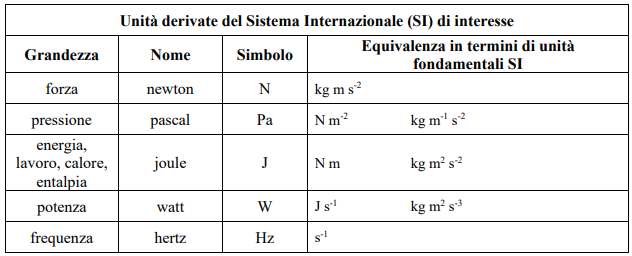
\includegraphics[height=5cm]{../L01/img10.PNG}
\end{center}
\begin{center}
    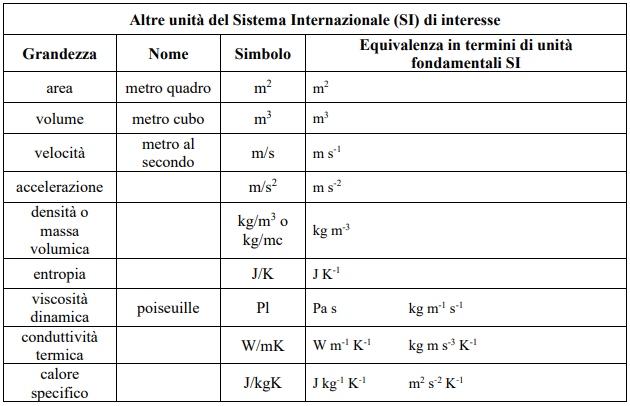
\includegraphics[height=7cm]{../L01/img11.PNG}
\end{center}
\begin{center}
    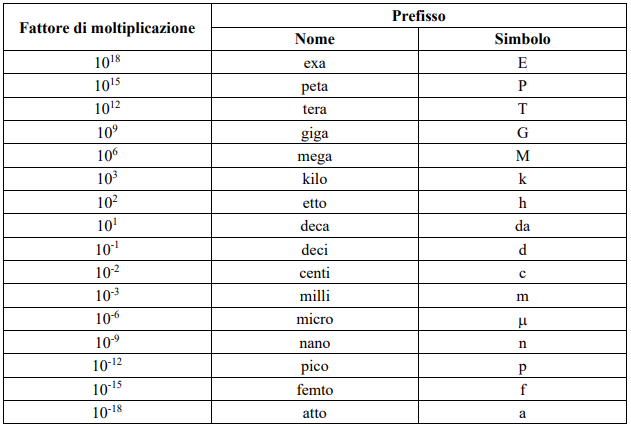
\includegraphics[height=5cm]{../L01/img12.PNG}
\end{center}
\begin{center}
    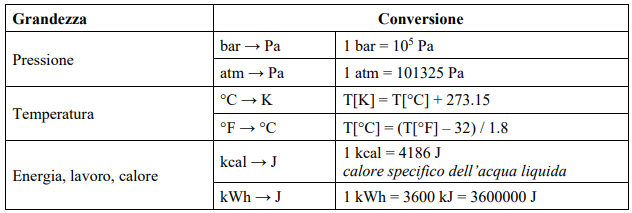
\includegraphics[height=5cm]{../L01/img13.PNG}
\end{center}
\section{Equazioni di bilancio per i sistemi chiusi}
Un \textbf{sistema chiuso} è un sistema per il quale non sono consentiti scambi di massa attraverso il suo contorno. Per tale sistema non è in uso applicare \textbf{equazioni di bilancio di massa} essendo implicita la sua conservazione nella definizione di sistema chiuso.\newline
\newline
Nelle soluzioni di problemi con sistemi chiusi le equazioni fondamentali sono \textbf{l'equazione di bilancio energetico} e \textbf{l'equazione di bilancio entropico} che assumono la forma:
\[
    \Delta U = Q^\leftarrow  -L^\rightarrow  
\]
\[
    \Delta S = S_Q + S_{irr}
\]
cioè la variazione di energia interna è pari alla differenza tra il calore entrante nel sistema e il lavoro ceduto dal sistema; la variazione di entropia è pari alla somma della entropia $S_Q$ entrante attraverso il contorno del sistema con il calore Q e della quantità $S_{irr}$ generata all'interno del sistema per irreversibilità. Questa ultima quantità è sempre positiva e tende a zero col tendere dei processi alla reversibilità. Inoltre il segno del termine $S_Q$ è sempre uguale al segno di $Q$.\newline
\newline
L'\textbf{energia interna} e l'\textbf{entropia} sono proprietà \textbf{estensive e additive}. Quindi dato un sistema $Z$ composto da due sottosistemi $A$ e $B$, posso scrivere:
\[
    \Delta U_Z = \Delta U_A + \Delta U_B = Q_Z^\leftarrow  - L_Z^\rightarrow  \;\;\;\;\;\;\;\;\;\;\Delta S_Z = \Delta S_A + \Delta S_B = S_{Q,Z} + S_{irr,Z}
\]
\ \newline
\newline
Se il \textbf{lavoro scambiato} è lavoro meccanico quasi-statico (internamente reversibile), è determinabile con l'espressione:
\[
    L = \int_{i}^{f} P dV
\]
Questa espressione è integrabile se è nota l'equazione della trasformazione ovvero la funzione:
\[
    P = P(V)
\]
\ \newline
Il \textbf{calore scambiato}, nell'ipotesi di trasformazione quasi-statica, può essere determinato avendo noto il calore specifico della trasformazione:
\[
    Q = M c_x (T_2-T_1)
\]
\ \newline
L'\textbf{energia interna} di un sistema in uno stato di equilibrio può essere espressa in funzione di altre proprietà intensive ed estensive specifiche del sistema come la temperatura, il volume specifico, la pressione. Particolarmente utili sono i due seguenti casi in cui è possibile esprimere in una forma analitica elementare il legame funzionale tra la variazione di energia interna tra due stati di equilibrio e la variazione di temperatura. \newline
\textbf{Gas perfetto}: $\Delta u = c_V (T_2 - T_1)$\newline
\textbf{Liquido incomprimibile perfetto}: $\Delta u = c(T_2-T_1)$\newline
Inoltre:
\begin{itemize}
    \item Per un sistema isolato $\Delta U_{isolato} = 0$.
    \item Per un sistema che subisce una trasformazione ciclica: $\Delta U_{ciclo} = 0$
\end{itemize}
\ \newline
\newline
Il caso di trasformazioni quasi-statiche a pressione costante o trasformazioni irreversibili in un sistema con stato iniziale e finale alla stessa pressione consente di scrivere l’equazione di bilancio energetico per il sistema chiuso come:
\[
    \Delta H = Q \;\;\;\;\;\;\;\;\;\;\;\;\;\;\;\text{dove $h = u + Pv$}\;
\]
Per esempio la miscelazione adiabatica e isobara di due sottosistemi produce uno stato finale caratterizzato da un valore di entalpia totale pari alla somma delle entalpia iniziale dei due sottosistemi. \newline
L'\textbf{entalpia specifica} di un sistema in uno stato di equilibrio può essere espressa
in funzione di altre proprietà intensive ed estensive specifiche del sistema come la
temperatura, il volume specifico, la pressione. Particolarmente utili sono i due seguenti casi
in cui è possibile esprimere in una forma analitica elementare il legame funzionale tra la
variazione di entalpia specifica tra due stati di equilibrio e la variazione di temperatura. \newline
\textbf{Gas perfetto}: $\Delta h = c_P (T_2 - T_1)$\newline
\textbf{Liquido incomprimibile perfetto}: $\Delta h = c(T_2-T_1) + v(P_2-P_1)$\newline
\newline
L'\textbf{entropia} è una proprietà del sistema e quindi dipende solo dallo stato del sistema: ne consegue che noti gli stati iniziale e finale di un processo, la determinazione della variazione di entropia prescinde dalla conoscenza di qualsiasi dettaglio del processo (ivi compresa la sua reversibilità). Particolarmente utili sono i due seguenti casi in cui è possibile esprimere in una forma analitica elementare il legame funzionale tra l'entropia e altre proprietà del sistema. Per il gas perfetto sono possibili 3 diverse espressioni che fanno uso di 3 diverse coppie di coordinate termodinamiche indipendenti. \newline
\textbf{Gas perfetto}:
\[
    \begin{matrix}
        \Delta s = c_P ln \frac{T_2}{T_1} - R^* ln \frac{P_2}{P_1} \;\;\;\;\;\;\;\;\;\;\;\;\;\;\;\Delta s = c_V ln \frac{T_2}{T_1} + R^* ln \frac{V_2}{V_1}\\
        \Delta s = c_V ln \frac{P_2}{P_1} + c_P ln \frac{V_2}{V_1}
    \end{matrix}
\]
\textbf{Liquido incomprimibile perfetto}: $\Delta s = c ln \frac{T_2}{T_1}$\newline
Inoltre:
\begin{itemize}
    \item Per definizione la variazione di entropia di un serbatoio di lavoro ($\Delta S_{SL}$) è nulla.
    \item Per definizione la variazione di entropia di un serbatoio di calore ($\Delta S_{SC}$) ha solo la componente reversibile, gli scambi avvengono con trasformazioni quasi-statiche (internamente reversibili).
    \item Un processo è impossibile da realizzare nel momento in cui $S_{irr} < 0$.
    \item La variazione di entrpia per una trasformazione reversibile è data da $\Delta S = \int_{i}^f \frac{1}{T} \delta Q_{rev}^\leftarrow$ (per i casi in cui $T$ è costante, allora $\Delta S = \frac{Q}{T}$).
    \item La variazione di entropia totale di un sistema isolato sede di trasformazioni termodinamiche è
    sempre maggiore di zero e tende a zero con il tendere dei processi alla reversibilità $\Delta S_{isolato} \geq 0$.
    \item $S_{irr} \geq 0$ è sempre maggiore di zero e il segno di $S_{Q}^\leftarrow $ è uguale al segno di $Q^\leftarrow$
\end{itemize}
\ \newline
\newline
\textbf{L’energia interna, l’entalpia e l’entropia} sono proprietà del sistema e quindi dipendono solo
dallo stato del sistema: ne consegue che noti gli stati iniziale e finale di un processo, la
determinazione della loro variazione prescinde dalla conoscenza di qualsiasi dettaglio del
processo (ivi compresa la sua reversibilità). Non è invece possibile determinare \textbf{il lavoro ed il
calore} scambiato dal sistema nel caso in cui si conoscano solo stato iniziale e finale e in tal caso non si ricorre pertanto alla scrittura del bilancio di energia (primo principio) e di entropia (secondo principio) che risulterebbero
indeterminati, ma si ricorre alle equazioni di stato (per i gas perfetti o per i liquidi incomprimibili perfetti\dots) che utilizzano solamente dati dello stato iniziale e finale.
\section{Stati monofase: equazioni di stato e trasformazioni}
Le sostanze nello stato monofase possono schematicamente essere suddivise in sostanze nello
stato aeriforme, liquido o solido. I modelli di equazioni di stato sono, in prima
approssimazione, ricondotti a modelli ideali o modelli reali.
\subsection{Gas ideali}
Le equazioni di stato dei \textbf{gas ideali} sono:
\[
    PV=MR^*T
\]
\[
    U=U(T) \;\;\;\;\;\;\;\;\;\;\;\;\Delta U = M c_V \Delta T \rightarrow \Delta u = c_V \Delta T
\]
La costante $R^*$ rappresenta la costante del gas ed è determinabile con la relazione:
\[
    R^* = \frac{R}{M_m}
\]
\[
    R=8314 [J/kmole K] =\text{costatne universale dei gas}\; \;\;\;\;\;\;\;\;\;\;M_m = \text{massa molare}\;
\]
\begin{center}
    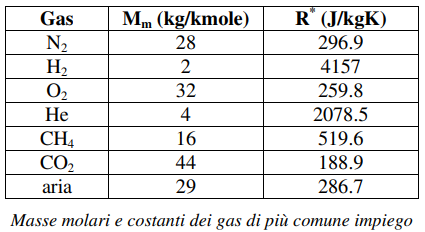
\includegraphics[height=3cm]{../NOTE SUGLI ESERCIZI/img1.PNG}
\end{center}
La grandezza $c_V$ rappresenta il calore specifico a volume costante funzione del gas e della sua
struttura molecolare. Qualora il calore specifico a volume costante possa assumersi indipendente dalla temperatura (e quindi costante) si parla di gas perfetto.
\subsection{Liquidi e solidi incomprimibili ideali}
Le equazioni di stato dei fluidi incomprimibili ideali (liquidi e solidi) sono:
\[
    v = costante
\]
\[
    U=U(T)  \;\;\;\;\;\;\;\;\;\;\;\;\Delta U = M c \Delta T \rightarrow \Delta u = c \Delta T
\]
dove $c$ è il calore specifico della sostanza.
\subsection{Gas reali}
Una possibile equazione di stato dei gas reali è:
\[
    Pv = ZRT
\]
dove $Z$ è il fattore di compressibilità. Tale coefficiente è determinabile attraverso il diagramma generalizzato che riposta il fattore di compressibilità in funzione della pressione e della temperatura ridotta. La pressione e la temperatura ridotte sono valori adimensionali ottenuti dalle relazioni:
\[
    P_R = \frac{P}{P_{cr}} \;\;\;\;\;\;\;\;\;\;\;\;\;\;\;T_R = \frac{T}{T_{cr}}
\]
in cui $P_{cr}$ e $T_{cr}$ rappresentano i valori di pressione e temperatura nello stato critico.
\begin{center}
    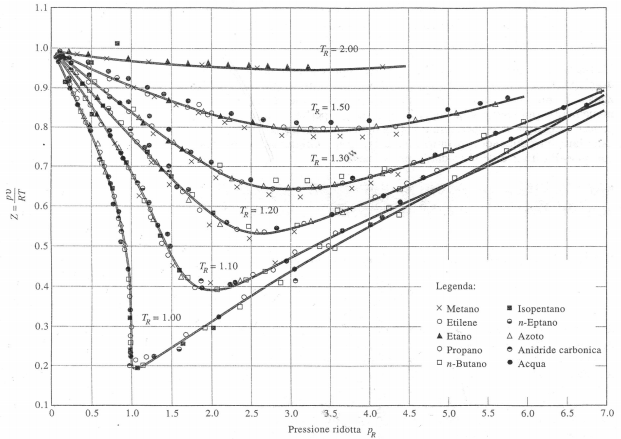
\includegraphics[height=5cm]{../NOTE SUGLI ESERCIZI/img2.PNG}
\end{center}
\subsection{Liquidi e solidi reali}
Le equazioni di stato dei liquidi e solidi reali sono formulate in forma differenziale:
\[
    dv = \beta v \cdot dT - K_Tv \cdot  dP
\]
\[
    \text{Coefficiente di dilatazione termica isobaro}\;\;\;\beta = \frac{1}{v} \left(\frac{\delta v}{\delta T}\right)_P
\]
\[
    \text{Coefficiente di comprimibilità isotermo}\;\;\;K_T = - \frac{1}{v} \left(\frac{\delta v}{\delta P}\right)_T
\]
Siccome $\beta$ e $K_T$ possono essere considerati costanti per ampi intervalli di temperatura e di pressione, la precedente relazione differenziale è integrabile e lo stato calcolabile.
\begin{center}
    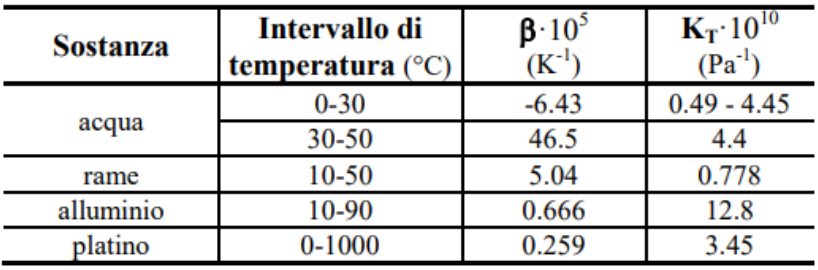
\includegraphics[height=3cm]{../NOTE SUGLI ESERCIZI/img3.PNG}
\end{center}
\subsection{Trasformazioni politropiche}
Le \textbf{trasformazioni politropiche} sono trasformazioni termodinamiche \textbf{internamente reversibili}
proprie dei \textbf{gas perfetti} e caratterizzate dall’avere un calore specifico $c_x$ \textbf{costante}.\newline
\newline
L’equazione della politropica in coordinate P,v risulta
\[
    Pv^n = costante \;\;\;\;\;\;\;\;\;\;\text{dove \textbf{l'indice della politropica} è}\;\;\;n = \frac{c_x - c_P}{c_x - c_V}
\]
Con l’ausilio dell’equazione di stato dei gas ideali è possibile ottenere espressioni
dell’equazione della politropica in coordinate T,P e T,v: 
\[
    P^{1-n}T^n = costante
\]
\[
    Tv^{n-1} = costante
\]
Si distinguono alcune trasformazioni elementari particolarmente utili tra le politropiche: 
\begin{center}
    \begin{tabular}{ |c|c|c|c| } 
        \hline
        Trasformazione & $c_x$ & $n = \frac{c_x - x_P}{c_x - c_V}$ \\
        \hline
        Isoterma ($T = costante$) & $\pm \infty$ & $1$ \\ 
        Isocora ($v = costante$) & $c_V$ & $\pm \infty$\\ 
        Isobara ($P = costante$) & $c_P$ & $0$\\ 
        Adiabatica ($q = costante$) & $0$ & $k= \frac{c_P}{c_V}$\\ 
        \hline
    \end{tabular}
\end{center}
\ \newline
Si ricorda che il \textbf{primo principio} è \textbf{sempre applicabile} ed essendo la trasformazione \textbf{quasi statica} vale inoltre sempre:
\[
    Q = \int_{1}^{2}TdS \;\;\;\;\;\;\;\;\;\;\;\;\;\;\;L=\int_{1}^{2}PdV
\]
Per la trasformazione \textbf{isoterma} (cioè con $n = 1$) il calore e il lavoro diventano:
\[
    Q = MT(s_2-s_2) \;\;\;\;\;\;\;\;\;\;\;\;\;\;\; L = P_1V_1 ln \left(\frac{V_1}{V_2}\right)
\]
Per le trasformazioni \textbf{isocore, isobare e adiabateche} (cioè con $n \neq 1$), invece, il calore e il lavoro diventano:
\[
    Q= Mc_x (T_2-T_1) \;\;\;\;\;\;\;\;\;\;\;\;\;\;\; L = \frac{P_1V_1}{n-1}\left[ 1 - \left(\frac{V_1}{V_2}\right)^{n-1}\right]
\]
Si suggerisce di ricorrere al calcolo degli integrali per determinare il lavoro e il calore
scambiato soltanto quando strettamente necessario. Essendo questi due termini comunque
legati tra loro dalla equazione di bilancio energetico. 
\section{Stati bifase: grandezze di stato e trasformazioni}
Lo \textbf{stato bifase} di una sostanza pura corrisponde alla coesistenza di due diverse fasi (solidoliquido, solido-vapore o liquido-vapore) in equilibrio tra loro (\textbf{stato eterogeneo}). Un sistema
in uno stato eterogeneo può essere pensato come un insieme di più sottosistemi in stati
omogenei. Si definisce \textbf{fase} di un sistema eterogeneo, il sottosistema omogeneo caratterizzato
dagli stessi valori di tutte le proprietà specifiche. Un sistema eterogeneo è in uno stato di
equilibrio se tutte le sue proprietà intensive hanno valori ovunque uguali (cioè sono uguali
per tutte le fasi). \newline
\newline
Si definisce \textbf{transizione di fase} la trasformazione che porta un sistema che si trova in uno
stato omogeneo a separarsi in due o più fasi.\newline
\newline
Un sistema monocomponente in uno stato bifase
ha un solo grado di libertà (nella regola di Gibbs: $V=1$). \newline
\newline
La pressione P e la temperatura T di un sistema monocomponente bifase sono infatti legate,
in qualsivoglia passaggio di stato, dalla relazione di Clausius-Clapeyron: 
\[
    \left(\frac{dP}{dT}\right)_{a \rightarrow b} = \frac{(s_a-s_b)}{(v_a-v_)b} \;\;\;\;\;\;\;\;\;\;\;\;\;\;\; \left( \frac{dP}{dT} \right)_{a \rightarrow  b} = \frac{(h_a-h_b)}{T(v_a-v_b)}
\]
Lo stato termodinamico di un sistema monocomponente bifase è quindi compiutamente
descritto da una variabile intensiva, essendo l'altra univocamente definita, e da una variabile
estensiva specifica o anche dalla coppia estensiva-estensiva. \newline
\newline
Di qui le varie rappresentazioni grafiche per il bifase: (P, v), (T,s), (P,h), (h,s) che contengono
sempre almeno una quantità estensiva specifica. 
\subsection{Proprietà termodinamiche estensive}
Faremo ora sempre assunzione allo stato bifase \textbf{liquido-vapore}.\newline
\newline
Indicando con $Z$ una generica grandezza estensiva, per una miscela bifase liquido-vapore si ha
\[
    Z = Z_l + Z_v
\]
cioè il valore della proprietà $Z$ per la miscela è pari alla somma del valore della proprietà estensiva della fase liquida $Z_l$ e della fase vapore $Z_v$. Adottando le grandezze estensive specifiche corrispondenti di $Z$, la relazione precedente può essere riscritta come 
\[
    Z = M_l z_l + M_v z_v
\]
dove $M_l$ e $M_v$ sono rispettivamente la massa di liquido e quella di vapore.\newline
\newline
Definendo \textbf{titolo} $x$ (espresso in massa) il rapporto tra la massa di vapore e la massa totale conenuta nel sistema:
\[
    x = \frac{M_v}{M_l+M_v}
\]
si ottiene la seguente relazione valida per ottenere il valore di qualsivoglia grandezza
estensiva specifica di un sistema bifase avendo noto il titolo: 
\[
    z = z_l(1-x) + xz_v \;\;\;\;\;\text{oppure}\;\;\;\;\; z = z_l + x z_{lv}
\]
dove $z_{lv}$ rappresenta la variazione della proprietà estensiva specifica nella transizione di fase. \newline
Con questa formula si possono esprimere \textbf{l'energia interna, il volume, l'entalpia e l'entropia specifiche} di un sistema bifase.\newline
\newline
Come si può notare per valutare il valore assunto da una grandezza estensiva specifica in un
sistema bifase è necessario conoscere il valore assunto dalla grandezza estensiva in
condizione di saturazione (liquido e vapore).
\subsection{Tabelle}
Questi valori sono riportati su tabelle. Le tabelle termodinamiche sono di due tipi: 
\begin{itemize}
    \item  tabelle dello \textbf{stato eterogeneo} dove sono riportate le proprietà termodinamiche del liquido
    saturo e del vapore saturo; il dato di ingresso (argomento) è o la temperatura o la pressione. \newline
    I dati in corrispondenza di questa sono : \newline
    \begin{itemize}
        \item la pressione o la temperatura di saturazione (univocamente definita); 
        \item il volume specifico del liquido e del vapore saturi e la loro differenza ($m^3/kg$); 
        \item la entalpia specifica del liquido e del vapore saturi e la loro differenza ($kJ/kg$);
        \item la entropia specifica del liquido e del vapore saturi e la loro differenza ($kJ/kgK$);
        \item l'energia interna specifica del liquido e del vapore saturi e la loro differenza ($kJ/kg$);
    \end{itemize}
    L' ultima grandezza non è sempre presente, ma è comunque valutabile dal legame
    esistente tra l’entalpia e l’energia interna ($h= u+ Pv$). 
    \item tabelle dello stato omogeneo che portano le proprietà del vapore surriscaldato; i dati di
    ingresso sono la temperatura e pressione (le due intensive che definiscono lo stato).\newline
    I dati in
    corrispondenza della particolare pressione sono:
    \begin{itemize}
        \item il volume specifico del vapore surriscaldato ($m^3/kg$);
        \item la entalpia specifica del vapore surriscaldato ($kJ/kg$);
        \item la entropia specifica del vapore surriscaldato ($kJ/kgK$);
        \item la energia interna specifica del vapore surriscaldato ($kJ/kg$);
    \end{itemize}
    L' ultima grandezza non è sempre presente, ma è comunque valutabile dal legame
    esistente tra l’entalpia e l’energia interna ($h= u+ Pv$). 
\end{itemize}
\ \newline
Qualora lo stato termodinamico di cui si stanno valutando le proprietà termodinamiche non
coincide con gli stati discreti riportati sulle tabelle è necessario eseguire una interpolazione
dei dati.\newline
\newline
L’utilizzo delle tabelle termodinamiche consente di valutare le proprietà di una sostanza,
normalmente, in condizioni di bifase liquido-vapore o nello stato di vapore surriscaldato.
L’analisi di alcuni processi può richiedere informazioni sulle proprietà termodinamiche in
stati diversi quali liquido sottoraffreddato o solido. \newline
In questi casi, se non sono disponibili tabelle specifiche, occorre ricorrere a valutazioni
approssimate che si ottengono con l’ausilio di equazioni di stato. \newline
Occorre porre attenzione che l’utilizzo contemporaneo di dati estratti da una tabella o valutati
con l’ausilio di relazioni approssimate richiede l’adozione dello stesso stato di riferimento
rispetto a cui valutare le grandezze di interesse (entalpia, entropia, energia interna, etc.). \newline
In prima approssimazione, ipotizzando che lo stato di riferimento sia lo stato triplo e fase
liquida, si possono seguire queste indicazioni: 
\begin{itemize}
    \item \textbf{Stato di liquido sottoraffreddato}:
    \begin{itemize}
        \item entalpia: \[
            h(T,P) = h(T,P_s) + v (P-P_s)
        \]
        \[
            h(T,P) \sim h(T,P_s)
        \]
        \item entropia: \[
            s(T,P) = s(T,P_s)
        \]
    \end{itemize}
    dove $h(T,P_s)$ e $s(T,P_s)$ sono l'entalpia e l'entropia dello stato di liquido saturo alla temperatura $T$ (e alla conseguente pressione di saturazione $P_s$).
    \item \textbf{Stato di solido (ghiaccio)}:
    \begin{itemize}
        \item entalpia:\[
            h(T,P) = h_{ls,t} + c_s(T-T_t) + v(P-P_t)
        \]
        \item entropia:\[
            s(T,P) = s_{lv,t} +c_s ln \frac{T}{T_t}
        \]
    \end{itemize}
    dove $h_{ls,t}$ e $s_{ls,t}$ sono l'entalpia e l'entropia associate alla transizione di fase liquido-solido allo stato triplo, $T_t$ e $P_t$ sono la temperatura e la pressione dello stato triplo mentre $c_s$ è il calore specifico della fase solida.\newline
    Per la transizione di fase liquido-solido dell'acqua ($T_t = 273.16 K, P_t = 0.6122kPa$) si ha:
    \[
        h_{ls,t} = -333kJ/kg
    \]
    \[
        s_{ls,t} = \frac{h_{ls,t}}{T_t} \;\;\;\;\;\;\;\;\;\;s_{ls,t} = \frac{-333}{273.16}kJ/kgK = -1.219 kJ/kgK
    \]
    \[
        c_s = 2.093 kJ/kgK
    \]
\end{itemize}
\section{Equazioni di bilancio per sistemi aperti}
Un \textbf{sistema aperto} è un sistema dal quale può \textbf{uscire} ed \textbf{entrare massa}.\newline
\newline
E' un \textbf{sistema fluente} è di conseguenza è necessario introdurre la \textbf{variabile di tempo} ($t$) e di conseguenza i \textbf{flussi di massa, di energia, di entropia,} etc.
\[
    \dot{m} \;\;\;\;\; \dot{E}\;\;\;\;\; \dot{U} \;\;\;\;\; \dot{H} \;\;\;\;\; \dot{S} \;\;\;\;\; \dot{Q} \;\;\;\;\; \dot{L}
\]
\ \newline
I \textbf{bilanci di massa, energia ed entropia} per i sistemi aperti sono la base per lo studio dei più
comuni componenti di interesse tecnico: pompe, compressori, turbine e scambiatori di calore. \newline
\newline
Le equazioni di bilancio, nella loro formulazione generale, sono:
\[
    \begin{cases}
        \frac{dM}{dt} = \sum_{k=1}^{n}\dot{m}_k^\leftarrow \\
        \frac{dE}{dt} = \sum_{k=1}^{n}\dot{m}_k^\leftarrow  \left(h + gz + \frac{w^2}{2}\right) + \dot{Q}^\leftarrow  - L_e^\rightarrow \\
        \frac{dS}{dt} = \sum_{k=1}^{n} \dot{m}_k^\leftarrow  s_k + \dot{S}_Q^\leftarrow + \dot{S}_{irr}
    \end{cases}
\]
Con $k$ si intendono le varie sezioni di passaggio.\newline
Con $\dot{L}_e^\rightarrow $ si intende il \textbf{lavoro d'elica}, cioè il lavoro scambiato per unità di tempo attraverso le sezioni non attraversate dalla massa.\newline 
Esiste anche il \textbf{lavoro di pulsione} $\dot{L}_P^\leftarrow $ che è il lavoro scambiato per unità di tempo attraverso le sezioni attraversate dalla massa e (per l'ingresso) si calcola come
\[
    L_{P,i}^\leftarrow  = M_i P v_i
\]
con $M_i$ la massa immessa nel sistema, $P$ la pressione costante che agisce su $M_i$, e $v_i$ il volume specifico della sessione di ingresso. Allo stesso modo si calcola il lavoro di pulsione per l'uscita.\newline
\newline
Un approccio tipico prevede come primo passo la stesura dei tre bilanci seguiti dalla semplificazione dei bilanci di energia e di entropia tramite il bilancio di massa.
\newline
\newline
\newline
\textbf{Regime stazionario con un ingresso e con un'uscita}\newline
Per regime stazionario o regime permanente si intende una condizione in cui le variazioni di massa, di energia e di entropia nel sistema sono nulle nel tempo:
\[
    \frac{dM}{dt} = 0 \;\;\;\;\;\;\;\;\;\; \frac{dE}{dt} = 0 \;\;\;\;\;\;\;\;\;\; \frac{dS}{dt} = 0
\]
Considerando inoltre una porzione di condotto delimitata da una sezione di \textbf{ingresso} (i) ed una di
\textbf{uscita} (u), i bilanci di massa, di energia e di entropia, in regime stazionario, si scrivono: 
\[
    \begin{cases}
        \dot{m}_i^\leftarrow = -\dot{m}_u^\leftarrow  = \dot{m}\\
        \frac{dE}{dt} = \dot{m}\left[ (h_i - h_u) + g(z_i-z_u) + \frac{w_i^2}{2} - \frac{w_u^2}{2}\right] + \dot{Q}^\leftarrow -L_e^\rightarrow = 0\\
        \dot{m}(s_i-s_u) + \dot{S}_Q^\leftarrow  + \dot{S}_{irr} = 0
    \end{cases}
\]
dove $\dot{m} = \rho w \Omega$ è la \textbf{portata} in massa del sistema ($\rho$ è la massa volumica, $\omega$ è la velocità media, $\Omega$ è l'area della sezione di passaggio, da notare che $\omega \Omega = \Gamma$ è la portata volumica e che $rho = VM$).
\subsection{Sistemi aperti notevoli}
\subsubsection{Macchina aperta}
La \textbf{machcina aperta} è un \textbf{dispositivo adiabatico} destinato a \textbf{scambiare lavoro} per il quale si ipotizzano trascurabili le variazioni di energia potenziale e di energia cinetica tra le sezioni di ingresso e di uscita.\newline
\newline
I bilanci diventano:
\[
    \begin{cases}
        \dot{m} (h_i - h_u) - \dot{L}_e^\rightarrow  = 0\\
        \dot{m} (s_i-s_u) + \dot{S}_{irr} = 0
    \end{cases}
\]
\begin{itemize}
    \item \textbf{Turbina}:\newline
    Una \textbf{turbina} produce lavoro, cioè genera potenza meccanica.\newline
    \newline
    Una turbina riduce il suo contenuto entalpico, la sua pressione e temperatura e aumenta il suo volume specifico.\newline
    \newline
    Nel caso di turbina il \textbf{lavoro d'elica uscente} è positivo, quindi l'entalpia in ingresso è maggiore dell'antalpia in uscita.\newline
    \newline
    Si chiama \textbf{rendimento isoentalpico} di una \textbf{macchina motrice aperta} (turbina) il rapporto fra la potenza realmente ottenuta e la potenza massima ottenibile in condizioni ideali a parità di condizioni in ingresso e a parità di pressione di fine espansione:
    \[
        \eta_T = \frac{\dot{L}_{reale}^\rightarrow }{\dot{L}_{ideale}^\rightarrow } = \frac{h_1 - h_{2'}}{h_1-h_2}
    \]
    dove per $\dot{L}_{reale}^\rightarrow $ si intende $\dot{L}_e$ e per $\dot{L}_{ideale}^\rightarrow $ si intende la potenza meccanica scambiata con un processo ideale (isoentropico).
    \item \textbf{Compressore e pompa}:\newline
    Se la macchina aperta assorbe lavoro dall'esterno, si parla di compressore o pompa a seconda del fluido di lavoro.\newline
    \newline
    Il meccanismo è opposto a quello della turbina.\newline
    \newline
    Nel caso di compressore o pompa il \textbf{lavoro d'elica uscente} è negativo.\newline
    \newline
    Si chiama \textbf{rendimento isoentropico} di una macchina operatrice aperta (compressore e pompa) il rapporto fra la potenza minima spesa in condizioni ideali e la potenza realmente spesa a parità di condizioni in ingresso e a parità di pressione di fine espansione:
    \[
        \eta_C = \frac{\dot{L}_{reale}^\rightarrow }{\dot{L}_{ideale}^\rightarrow } = \frac{h_1-h_2}{h_1-h_{2'}} 
    \]
    dove per $\dot{L}_{reale}^\rightarrow $ si intende $\dot{L}_e$ e per $\dot{L}_{ideale}^\rightarrow $ si intende la potenza meccanica scambiata con un processo ideale (isoentropico).
\end{itemize}
\subsubsection{Scambiatori di calore}
Lo \textbf{scambiatore di calora} è un dispositivo destinato a \textbf{scambiare calre} e che \textbf{non scambia lavoro} per il quale si ipotizzano trascurabili le variazioni di energia potenziale e di energia cinetica tra le sezioni di ingresso e di uscita.\newline
\newline
I bilanci diventano:
\[
    \begin{cases}
        \dot{m}(h_i - h_u) + \dot{Q}^\leftarrow  = 0\\
        \dot{m}(s_i-s_u) + \dot{S}_{Q}^\leftarrow + \dot{S}_{irr} =0 
    \end{cases}
\]
\subsubsection{Casi minori}
\begin{itemize}
    \item I \textbf{diffusori} ($w \searrow$) e gli \textbf{ugelli} ($w \nearrow$) sono sistemi aperti stazionari che operano \textbf{senza scambio di lavoro nè calore} per i quali si ipotizzano trascurabili le variazioni di energia potenziale tra le sezioni di ingresso e di uscita.\newline
    La differenza fra diffusore e ugello dipende se lo stato di ingresso si trova a una velocità di ingresso maggiore (diffusore) rispetto a quella d'uscita o viceversa (ugello).\newline
    \newline
    I bilanci diventano:
    \[
        \begin{cases}
            \left[(h_i-h_u) + \frac{w_i^2 - w_u^2}{2}\right] = 0\\
            \dot{m} (s_i-s_u) + \dot{S}_{irr} =0 
        \end{cases}
    \]
    \item La \textbf{valvola di laminazione} è un \textbf{dispositivo adiabatico} che \textbf{non scambia lavoro} per il quale si ipotizzano trascurabili le variazioni di energia potenziale e di energia cinetica tra le sezioni di ingresso e di uscita. Si ottiene un processo detto di \textbf{laminazione isoentalpica} (cioè in cui l'entalpia in ingresso e in uscita sono identiche).\newline
    A livello pratico ciò che succede in questo tipo di sistemi è che la pressione scende fra ingresso e uscita (come se ci fosse uno strozzamenteo).\newline
    \newline
    I bilanci diventano:
    \[
        \begin{cases}
            (h_i- h_u) = 0\\
            \dot{m} (s_i-s_u) + \dot{S}_{irr} = 0
        \end{cases}
    \]
\end{itemize}
\section{Macchine termodinamiche}
Con il termine di \textbf{macchina termodinamica} si intende un sistema composto da un opportuna
combinazione di sottosistemi elementari (serbatoio di calore, serbatoio di lavoro e macchina
ciclica) che ha come funzione o la conversione termodinamica di energia termica in lavoro
(\textbf{macchina termodinamica motrice}) o il trasferimento di energia termica da uno o più serbatoi
di calore a temperatura inferiore a uno o più serbatoi di calore a temperatura superiore
(\textbf{macchina termodinamica operatrice}). \newline
\newline
Per \textbf{serbatoio di calore} si intende un sistema termodinamico che scambia \textbf{solo calore} con l'esterno senza alterare il suo stato termodinamico (cioè la temperatura e la pressione del serbatoio rimangono costanti, il suo stato non cambia); gli scambi avvvengono con trasformazioni quasi-statiche (\textbf{internamente reversibili}). Questa definizione di serbatoio è sinonimo di un sistema \textbf{a massa infinita}.\newline
\newline
Per \textbf{serbatoio di lavoro} si intende un sistema termodinamico che scambia \textbf{solo lavoro} con l'esterno senza alterare il suo stato termodinamico; gli scambi avvengono con trasformazioni quasi-statiche (\textbf{internamente reversibili}).
\subsection{macchina motrice con sorgenti a temperatura cosante}
\begin{center}
    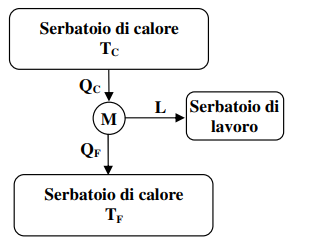
\includegraphics[height=5cm]{../NOTE SUGLI ESERCIZI/img4.PNG}
\end{center}
Vediamo la macchina motrice da un punto di vista analitico.\newline
Dalle equazioni di bilancio otteniamo:
\[
    \begin{cases}
        \Delta U_Z = 0\\ \Delta S_Z = S_{irr}
    \end{cases} \;\;\;\;\;\;\;\;\;\;\;\;\;\;\; \begin{cases}
        \Delta U_C + \Delta U_F + \Delta U_{SL} + \Delta U_M = 0 \\
        \Delta S_C + \Delta S_F + \Delta S_{SL} + \Delta S_M = S_{irr}
    \end{cases}
\]
Osservando i singoli sottosistemi otteniamo:
\[
    \begin{cases}
        \Delta U_C = Q_C^\leftarrow \\ \Delta S_C = \frac{Q_C^\leftarrow }{T_C}
    \end{cases} \;\;\;\;\; \begin{cases}
        \Delta U_F = Q_F^\leftarrow \\ \Delta S_F = \frac{Q_F^\leftarrow}{T_F}
    \end{cases} \;\;\;\;\; \begin{cases}
        \Delta U_{SL} = - L_{SL}^\rightarrow \\ \Delta S_{SL} = 0
    \end{cases} \;\;\;\;\; \begin{cases}
        \Delta U_M = 0\\ \Delta S_M = 0
    \end{cases}
\]
Dai bilanci energetico ed entropico della macchina termodinamica motrice illustrata in figura
e che è caratterizzata da operare con serbatoi di calore a temperatura costante $T_S$ e $T_F$, si
ottiene: 
\[
    \begin{cases}
        Q_C^\leftarrow  + Q_F^\leftarrow  - L_{SL}^\rightarrow = 0\\
        \frac{Q_C^\leftarrow}{T_C} + \frac{Q_C^\leftarrow}{T_F} = S_{irr}
    \end{cases}\;\;\;\;\;\longrightarrow\;\;\;\;\;\begin{cases}
        -Q_C + L + Q_F = 0\\
        - \frac{Q_C}{T_C} + \frac{Q_F}{T_F} = S_{irr}
    \end{cases}
\]
\ \newline
L’analisi termodinamica di una macchina termodinamica motrice richiede spesso di separare
l’analisi della macchina ideale (reversibile) che consente di massimizzare il lavoro prodotto
da quella reale (irreversibile). \newline
Nel caso di macchina termodinamica motrice \textbf{ideale}, o reversibile, si ottiene: 
\[
    L_{rev} = Q_C \left(1- \frac{T_F}{T_C}\right)
\]
\[
    \eta_{rev} = 1- \frac{T_F}{T_C}
\]
\ \newline
Nel caso di macchina termodinamica motrice \textbf{reale}, o irreversibile, si ottiene:
\[
    L  = Q_C \left(1- \frac{T_F}{T_C}\right) - T_FS_{irr}
\]
\[
    \eta = \frac{L}{Q_C} = 1-\frac{T_F}{T_C} - \frac{T_F S_{irr}}{Q_C}
\]
\ \newline
Questi concetti consentono di introdurre il concetto di \textbf{lavoro perso} (o dissipato):
\[
    L_P = L_{rev} - L \;\;\;\;\;\;\;\;\;\;\;\;\;\;\;L_{P} = T_FS_{irr}
\]
che rappresenta l’energia che il sistema termodinamico reale non è in grado di convertire in
lavoro utile a causa di una non-idealità intrinseca del processo di conversione analizzato.
\subsection{macchina operatrice con sorgenti a temperatura costante}
\begin{center}
    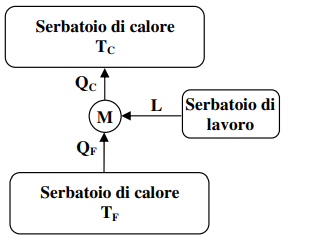
\includegraphics[height=5cm]{../NOTE SUGLI ESERCIZI/img5.PNG}
\end{center}
Vediamo la macchina operatrice da un punto di vista analitico.\newline
Dalle equazioni di bilancio otteniamo:
\[
    \begin{cases}
        \Delta U_Z = 0\\ \Delta S_Z = S_{irr}
    \end{cases} \;\;\;\;\;\;\;\;\;\;\;\;\;\;\; \begin{cases}
        \Delta U_C + \Delta U_F + \Delta U_{SL} + \Delta U_M = 0 \\
        \Delta S_C + \Delta S_F + \Delta S_{SL} + \Delta S_M = S_{irr}
    \end{cases}
\]
Osservando i singoli sottosistemi otteniamo:
\[
    \begin{cases}
        \Delta U_C = Q_C^\leftarrow \\ \Delta S_C = \frac{Q_C^\leftarrow }{T_C}
    \end{cases} \;\;\;\;\; \begin{cases}
        \Delta U_F = Q_F^\leftarrow \\ \Delta S_F = \frac{Q_F^\leftarrow}{T_F}
    \end{cases} \;\;\;\;\; \begin{cases}
        \Delta U_{SL} = - L_{SL}^\rightarrow \\ \Delta S_{SL} = 0
    \end{cases} \;\;\;\;\; \begin{cases}
        \Delta U_M = 0\\ \Delta S_M = 0
    \end{cases}
\]
Dai bilanci energetico ed entropico della macchina termodinamica operatrice illustrata in
figura e che è caratterizzata da operare con serbatoi di calore a temperatura costante $T_C$ e $T_F$ si
ottiene:
\[
    \begin{cases}
        Q_C^\leftarrow  + Q_F^\leftarrow  - L_{SL}^\rightarrow  = 0\\
        \frac{Q_C^\leftarrow}{T_C} + \frac{Q_F^\leftarrow}{T_F} = S_{irr}
    \end{cases} \;\;\;\;\;\longrightarrow\;\;\;\;\;\begin{cases}
        +Q_C - L - Q_F = 0\\
        + \frac{Q_C}{T_C} - \frac{Q_F}{T_F} = S_{irr}
    \end{cases}
\]
Rispetto alla macchina motrice è differente l’equazione di bilancio entropico in quanto
cambiano i segni dei contributi associati ai serbatoi di calore e di lavoro.\newline
\newline
Anche in questo caso si separa l’analisi della macchina termodinamica ideale (reversibile) per
la quale viene minimizzato il lavoro necessario per realizzare il processo, rispetto alla
macchina termodinamica operatrice reale (o irreversibile). \newline
Nel caso di macchina termodinamica operatrice \textbf{ideale}, o reversibile, si ottengono le due
relazioni: 
\[
    L_{rev,F} = Q_F\left(\frac{T_C}{T_F}-1\right) \;\;\;\;\;\;\;\;\;\;\;\;\;\;\; L_{rev,PC} = Q-C \left(1- \frac{T_F}{T_C}\right)
\]
che si differenziano per il fatto di consentire la valutazione del lavoro assorbito in funzione
del calore prelevato dalla sorgente inferiore (analisi tipica della macchina \textbf{frigorifera}) o del
lavoro assorbito in funzione del calore ceduto alla sorgente di lavoro (analisi tipica della
\textbf{pompa di calore}).
\newline
\newline
Nel caso di macchina termodinamica operatrice \textbf{reale}, o irreversibile, si ottengono: 
\[
    L = Q_F\left(\frac{T_C}{T_F}-1\right) + T_C S_{irr} \;\;\;\;\;\;\;\;\;\;\;\;\;\;\; L = Q_C \left(1- \frac{T_F}{T_C}\right) + T_F S_{irr}
\]
Il lavoro assorbito è in questo caso maggiore rispetto a quello assorbito nel caso ideale. \newline
\newline
Come parametro di merito si introduce, per le macchine termodinamiche operatrici
l’efficienza $\epsilon$ (anche detto COP). \newline
\newline
Nel caso di funzionamento come macchina \textbf{frigorifera} si ha: 
\[
    \epsilon_{f,rev} = \frac{T_F}{T_C-T_F} \;\;\;\;\;\;\;\;\;\;\;\;\;\;\; \epsilon_{f} = \frac{Q_F}{L} = \frac{T_F}{T_C-T_F + \frac{T_CT_FS_{irr}}{Q_F}}
\]
Nel caso di funzionamento come \textbf{pompa di calore} si ha:
\[
    \epsilon_{PC, rev} = \frac{T_C}{T_C-T_F} \;\;\;\;\;\;\;\;\;\;\;\;\;\;\; \epsilon_{PC} = \frac{Q_C}{L} = \frac{T_C}{T_C-T_F + \frac{T_CT_FS_{irr}}{Q_C}}
\]
\ \newline
Legame fra efficienza della macchina frigorifera e della pompa di calore:
\[
    \epsilon_P = \frac{Q_C}{L} = \frac{Q_F + L}{L} = \epsilon_F +1
\]
\subsection{Macchina motrice con serbatoio caldo a massa finita}
Vedi teoria per un esempio.
\subsection{Rendimento di secondo principio}
Il rendimento di una macchina termodinamica motrice e l’efficienza (o il COP) di una
macchina termodinamica operatrice rappresentano il cosiddetto \textbf{rendimento di primo
principio} che è un indice della capacità del processo di conversione dell’energia di soddisfare
gli obiettivi a fronte di una certa spesa energetica. \newline
\newline
Viene anche introdotto il concetto di \textbf{rendimento di secondo principio} che rappresenta la
capacità di un processo reale di avvicinarsi alle prestazioni del processo ideale (che nel caso
termodinamico è il processo reversibile per il quale non si ha produzione di entropia per
irreversibilità). Per la macchina termodinamica motrice e per la macchina termodinamica
operatrice (frigorifera o pompa di calore) si ha: 
\[
    \eta_{II} = \frac{L}{L_{rev}} \;\;\;\;\;\;\;\;\;\;\;\;\;\;\; \eta_{II} = \left(\frac{\eta}{\eta_{rev}}\right)_{Tc, Qc, Tf}
\]
\[
    \eta_{II} = \frac{L_{rev}}{L} \;\;\;\;\;\;\;\;\;\;\;\;\;\;\; \eta_{II} = \left(\frac{\epsilon}{\epsilon_{rev}}\right)_{Tc,Tf,Qf}
\]
\ \newline
\textbf{oss.} i risultati che sono stati ottenuti valgono solo per macchine termodinamiche con
sorgenti a temperatura costante. 
\section{Cicli a gas e a vapore}
Una prima classificazione dei cicli termodinamici distingue tra cicli a gas e cicli a vapore.
L’analisi termodinamica dei cicli richiede la valutazione degli stati termodinamici dei punti
caratteristici del ciclo al fine di determinare le potenze termiche e meccaniche scambiate tra
macchina ciclica ed i serbatoi di calore e lavoro.
\subsection{Cicli a gas}
\subsubsection{Ciclo Joule-Brayton}
ciclo simmetrico a gas che nella sua realizzazione ideale è costituito da
due trasformazione isoentropiche e due trasformazioni isobare. Questo ciclo può essere
realizzato anche come macchina operatrice. \newline
Per il ciclo Joule Brayton viene definito il rapporto delle pressioni:
\[
    r_P = \frac{P_{max}}{P_{min}}
\]
mentre il rendimento termodinamico assume l'espressione:
\[
    \eta_{JB} = 1- \frac{T_1}{T_2} \;\;\;\;\;\;\;\;\;\;\eta_{JB} = 1- \frac{1}{r_P^{\frac{k-1}{k}}}
\]
\subsubsection{Ciclo Otto}
ciclo simmetrico a gas che nella sua realizzazione ideale è costituito da due
trasformazione isoentropiche e due trasformazioni isovolumiche. \newline
Per il ciclo Otto viene definito il rapporto di compressione volumetrico:
\[
    r_V = \frac{V_1}{V_2}
\]
mentre il rendimento termodinamico assume l'espressione:
\[
    \eta_{O} = 1- \frac{T_1}{T_2} \;\;\;\;\;\;\;\;\;\; \eta_{O} = 1- \frac{1}{r_V^{k-1}}
\]
\subsubsection{Ciclo Diesel}
ciclo non simmetrico a gas che nella sua realizzazione ideale è costituito da due
trasformazione isoentropiche, una trasformazione isobara e una trasformazioni isovolumica. \newline
Per il ciclo Diesel vengono definiti il rapporto di compressione volumetrico e il rapporto di
combustione: 
\[
    r= \frac{V_1}{V_2} \;\;\;\;\;\;\;\;\;\;z = \frac{V_3}{V_2}
\]
mentre il rendimento termodinamico assume l'espressione:
\[
    \eta = 1- \frac{1}{r^{k-1}} \frac{1}{k} \frac{(z^k - 1)}{(z-1)}
\]
\subsection{Cicli a vapore}
\subsubsection{Ciclo Rankine}
ciclo che nella sua realizzazione ideale è costituito da due trasformazione
isoentropiche e due trasformazioni isobare. Durante le due trasformazioni isobare si realizza
la transizione di fase. \newline
Il rendimento termodinamico è definito come:
\[
    \eta = \frac{\dot{L}}{\dot{Q}_C}
\]
\subsubsection{Ciclo frigorifero a vapore}
ciclo che nella sua realizzazione ideale è costituito da due
trasformazioni isobare, una trasformazione isoentropica e una trasformazione isoentalpica
irreversibile. \newline
L'efficienza frigorifera (detta anche $COP_F$) e l'efficienza della pompa di calore (detta anche $COP_{PC}$) sono definite come:
\[
    \epsilon_F = \frac{\dot{Q}_F}{\dot{L}} \;\;\;\;\;\;\;\;\;\;\epsilon_{PC} = \frac{\dot{Q}_C}{\dot{L}}
\]
Per l'analisi dei cicli termodinamici a vapore occorre utilizzare le tabelle termodinamiche con le proprietà delle sostanze.
\subsection{Osservazioni}
\begin{itemize}
    \item Per la determinazione del rendimento termodinamico di un ciclo non noto ci viene utile la definizione di rendimento nella forma:
    \[
        \eta = 1- \frac{Q_F}{Q_C}
    \]
    osservando che le trasformazioni per le quali, nel piano T- s, si ha un aumento di entropia
    comportano un trasferimento di calore alla macchina ciclica (calore entrante) mentre
    viceversa le trasformazioni per le quali si ha una riduzione di entropia sono associate a una
    cessione di calore dalla macchina ciclica. (es. isobara è calore entrante ($Q_C$), isocora è calore uscente ($Q_F$), le trasformazioni isoentropiche sono adiabatiche e quindi non hanno trasferimento di calore).
    \item  trasformazione \textbf{isoentropica} significa trasformazione adiabatica reversibile.
\end{itemize}